\section{Introducción}
% Resumen, Antecedentes, Situación actual, Alcance

% Se empieza mencionando la interación de la persona con el ordenador.  Se
% cuenta como ha ido evolucionando hasta utilzar los dispositivos de entrada
% clásicos como el teclado, ratón o gamepads.
\begin{frame}
  \frametitle{Dispositivos de entrada clásicos}
  La interacción con los ordenadores generalmente se realiza a través de
  dispositivos de entrada como el \alert{teclado, ratón o \textit{gamepads}} en
  el caso de los videojuegos.

  \vspace{0.4cm}

  \centering
  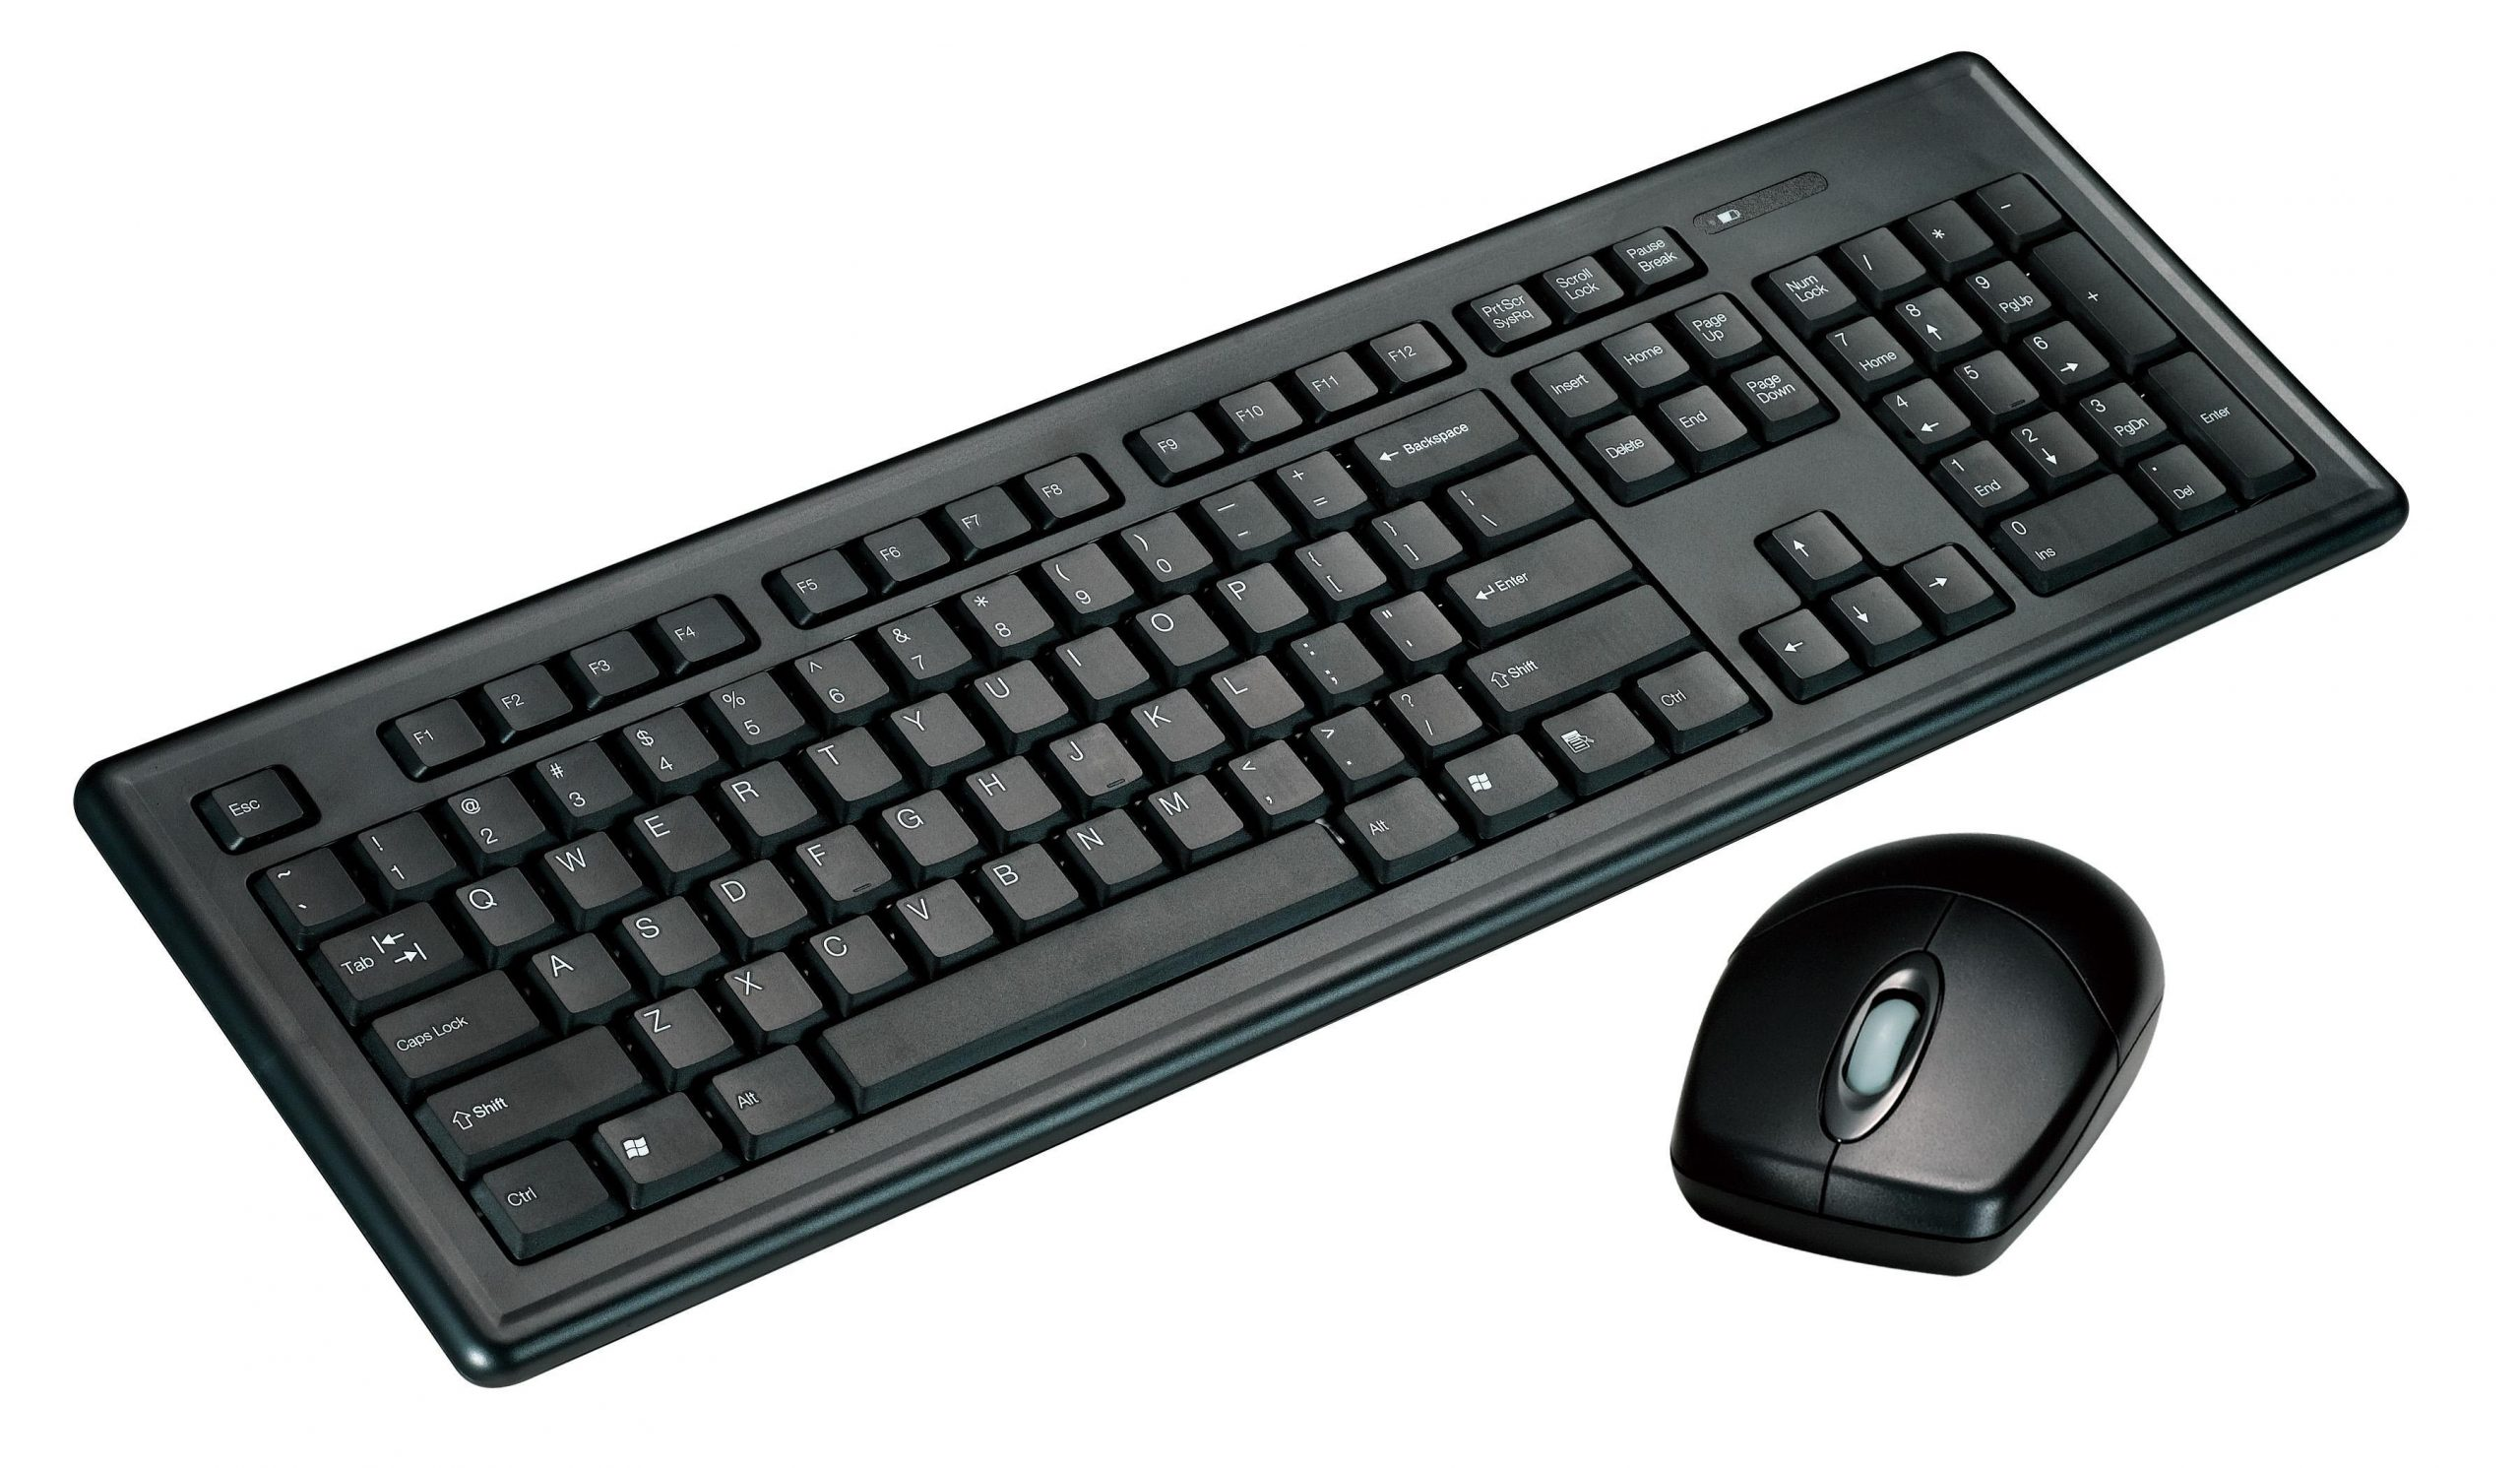
\includegraphics[width=0.5\textwidth]{pre/imgs/intro/keymouse.jpg}
  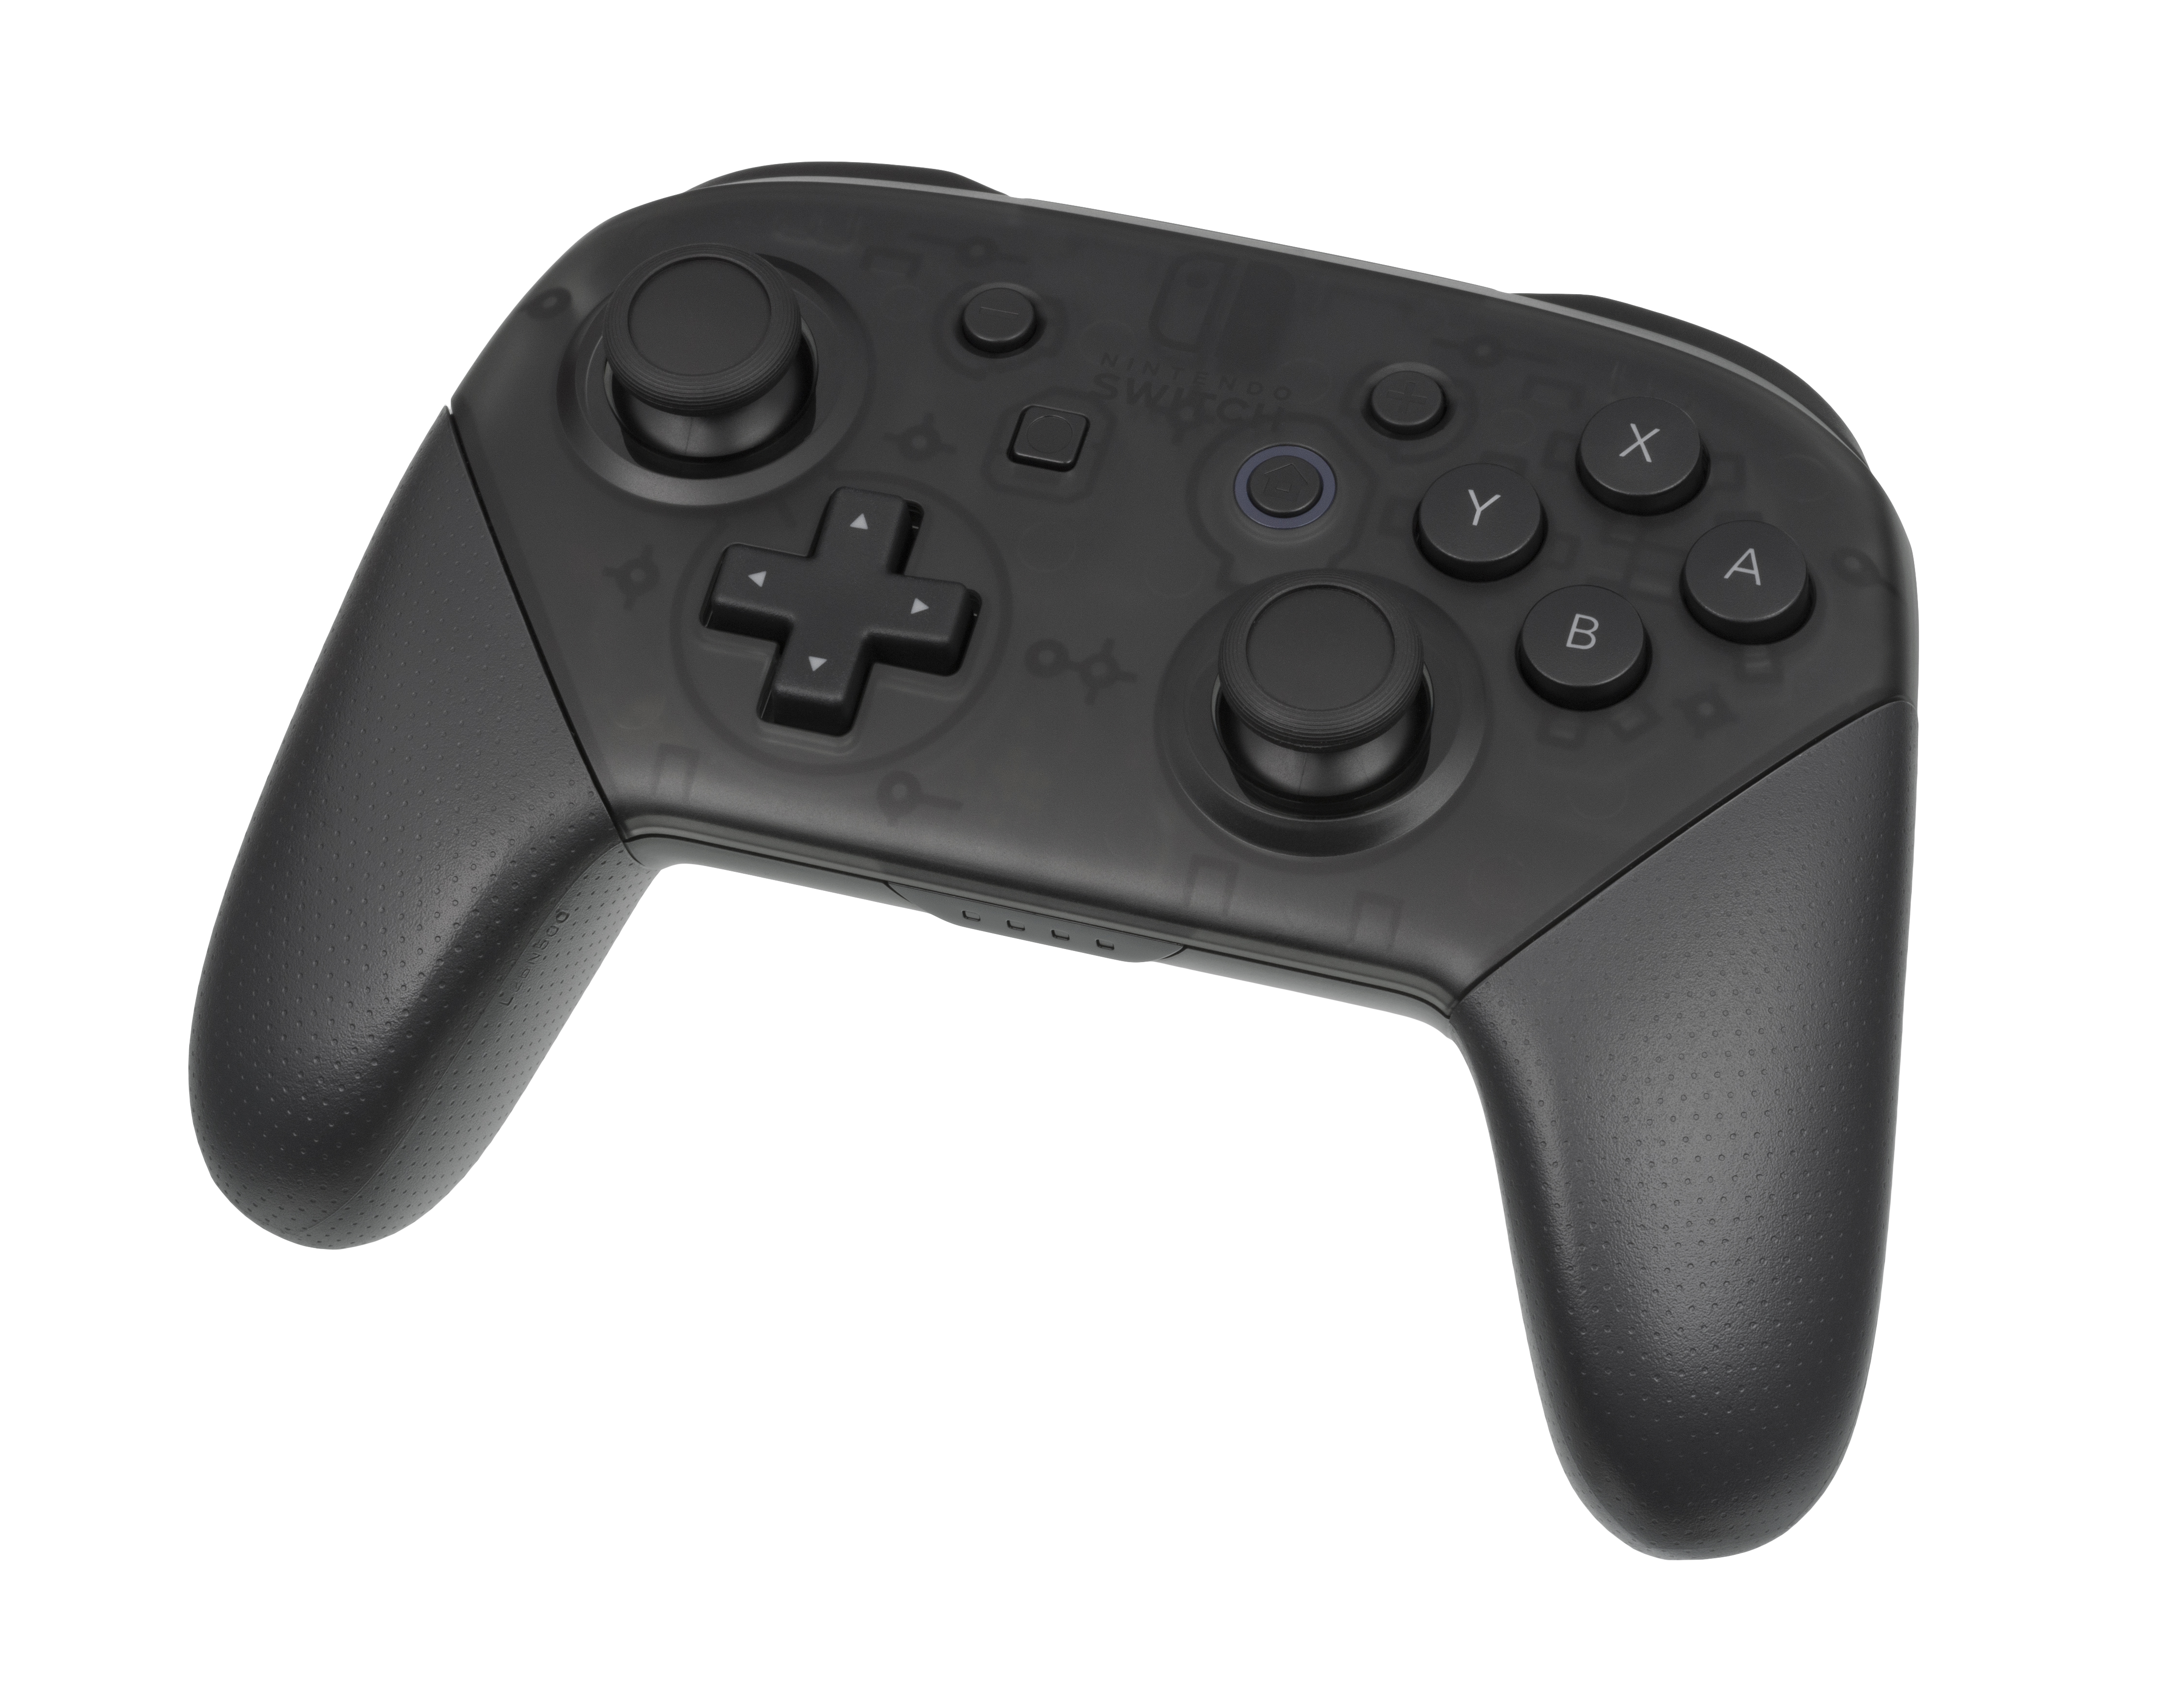
\includegraphics[width=0.4\textwidth]{pre/imgs/intro/gamepad.jpg}
\end{frame}

% Mencionamos los dispositivos más especializados como los
\begin{frame}
  \frametitle{Situación actual}

  Con el avance de la tecnología, han surgido nuevos dispositivos de entrada
  que permiten una interacción más natural y fluida con los sistemas. Ejemplos
  de esto son el \alert{Kinect}, la consola \alert{Nintendo Wii} o el sistema
  seguido por \alert{Just Dance Now}.

  \centering

  %\fbox{
  \begin{minipage}[c][0.4\textheight][c]{0.5\textwidth}
    \centering
    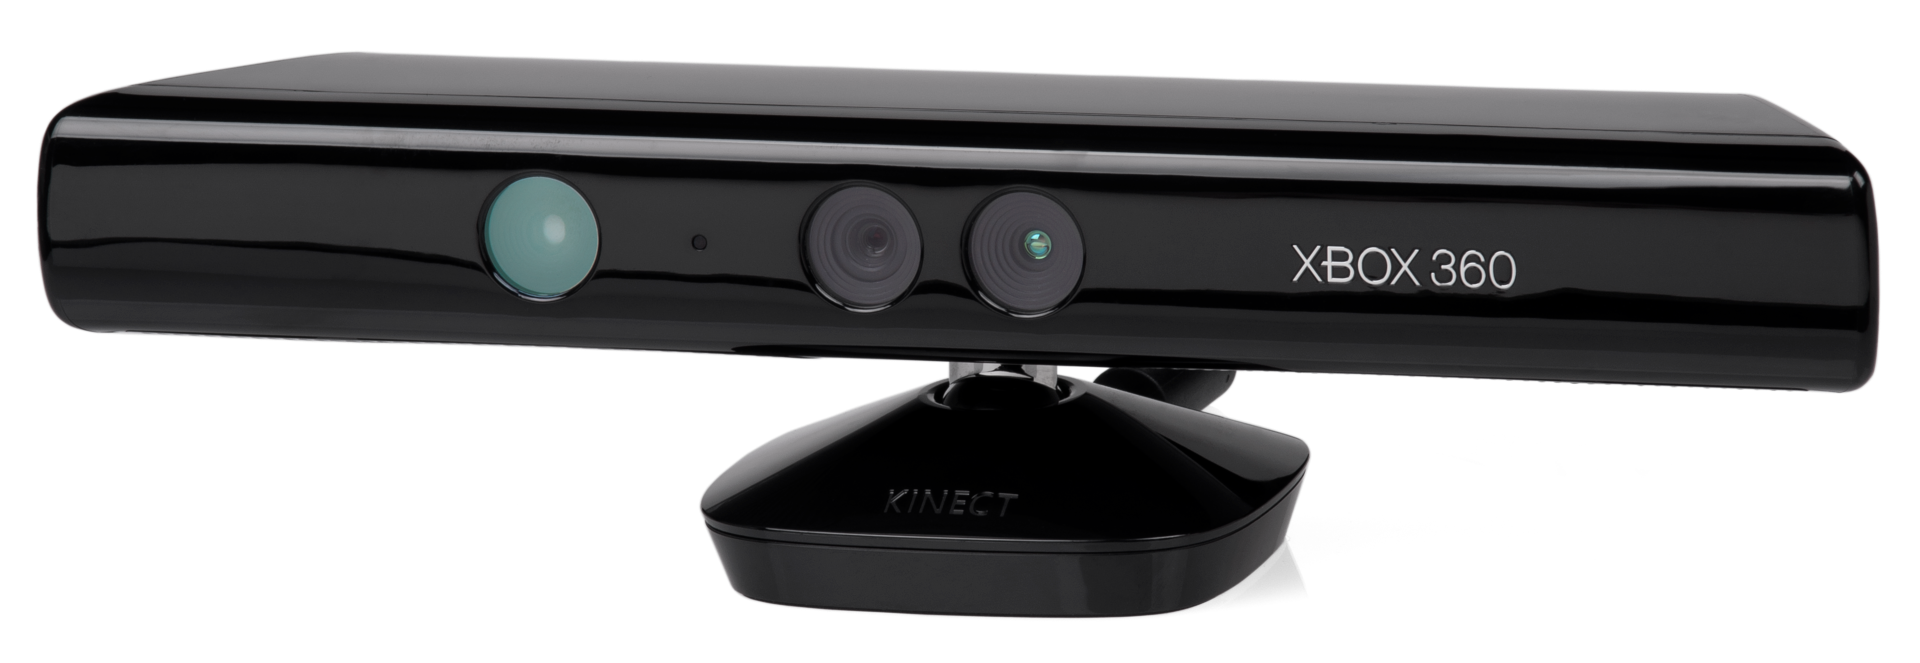
\includegraphics[width=\textwidth]{pre/imgs/intro/kinect.png}
  \end{minipage}
  %}\fbox{
  \begin{minipage}[c][0.4\textheight][c]{0.3\textwidth}
    \centering
    
\includegraphics[height=0.4\textheight]{pre/imgs/intro/wii.png}
  \end{minipage}
  %}

\end{frame}
